%XeTeX
\documentclass[a4paper, 11pt, titlepage]{report}

%Font stuff
\usepackage{fontspec}
\setmainfont[Ligatures={TeX}]{Adobe Caslon Pro}
\newfontfamily\crimsonfont[Ligatures={TeX}]{Crimson}
%1.5 line spacing
\usepackage{setspace}
\onehalfspacing
%\renewcommand{\baselinestretch}{1.2}

%New line between paragraphs, not indentation
\usepackage[parfill]{parskip}

%Make it look good
\usepackage{microtype}
%Colours
\usepackage{xcolor}
\definecolor{brown}{HTML}{85661E}
\definecolor{maroon}{HTML}{800B0B}
\definecolor{navyblue}{HTML}{1E5A9C}

%Margins
\usepackage[top=2.2cm, bottom=2.2cm, left=2.5cm, right=2.5cm]{geometry}

%Tables
\usepackage{tabularx}

%For appendix
\usepackage[titletoc, title]{appendix}
%Maths
\usepackage{mathtools}
%\usepackage{xfrac} %For sfrac
\usepackage{unicode-math}
 %Use XITS for the TOC as LMM causes hyperref to make buggy click boxes
%\setmathfont{xits-math.otf}
%Footnotes at the bottom
\usepackage[bottom]{footmisc}

%PDF hyperlinks
\usepackage{hyperref}
\hypersetup{
     colorlinks		= true,
     citecolor		= maroon,
     linkcolor		= maroon,
     urlcolor		= navyblue,
     bookmarksopen	= false,
     pdfpagemode	= UseNone,
     pdftitle		= {CITS3001 Assignment Report - 2014},
     pdfauthor		= {Jeremy Tan, 20933708},
     pdfsubject	= {Assignment 2014 - Threes}
}

%Tables
\usepackage{float}
\usepackage{caption}
\usepackage{tablefootnote}
\captionsetup[table]{skip=7pt}

%Headings
\usepackage{fancyhdr}
\pagestyle{fancy}
\addtolength{\headheight}{2.5pt}
\renewcommand{\chaptermark}[1]{\markboth{\thechapter~~#1}{}}
\renewcommand{\sectionmark}[1]{\markright{\thesection~~#1}{}}
\lhead{\bfseries \leftmark}
\rhead{\bfseries \thepage}
\cfoot{}

%Chapter marks
\usepackage[compact]{titlesec}
\titlespacing*{\chapter}{0pt}{-50pt}{0pt}
\titleformat{\chapter}
	{\normalfont\LARGE\bfseries}{\thechapter.}{0.8em}{}
	
%Importing files
\usepackage{import}
\usepackage{pgf}
\usepackage{tikz}
%\usepackage{lipsum}

% Sub/Superscripting
\newcommand{\ts}{\textsuperscript}
\newcommand{\tu}{\textsubscript}

%Code
\usepackage{listings}
\usepackage{accsupp}% http://ctan.org/pkg/accsupp
\newcommand{\emptyaccsupp}[1]{\BeginAccSupp{ActualText={}}#1\EndAccSupp{}}
\usepackage{xcolor}
\definecolor{mygreen}{rgb}{0,0.6,0}
\definecolor{mygray}{rgb}{0.5,0.5,0.5}
\definecolor{mymauve}{rgb}{0.58,0,0.82}
\lstset{
  basicstyle=\ttfamily\footnotesize\footnotesize,        % the size of the fonts that are used for the code
  breakatwhitespace=false,         % sets if automatic breaks should only happen at whitespace
  breaklines=true,                 % sets automatic line breaking
  captionpos=b,                    % sets the caption-position to bottom
  commentstyle=\color{mygreen},    % comment style
  deletekeywords={...},            % if you want to delete keywords from the given language
  escapeinside={\%*}{*)},          % if you want to add LaTeX within your code
  extendedchars=true,              % lets you use non-ASCII characters; for 8-bits encodings only, does not work with UTF-8
  frame=single,                    % adds a frame around the code
  columns=true,
  keepspaces=true,                 % keeps spaces in text, useful for keeping indentation of code (possibly needs columns=flexible)
  keywordstyle=\color{blue},       % keyword style
  morekeywords={*,...},            % if you want to add more keywords to the set
  numbers=left,                    % where to put the line-numbers; possible values are (none, left, right)
  numbersep=5pt,                   % how far the line-numbers are from the code
  numberstyle=\tiny\color{mygray}\emptyaccsupp, % the style that is used for the line-numbers
  rulecolor=\color{black},         % if not set, the frame-color may be changed on line-breaks within not-black text (e.g. comments (green here))
  showspaces=false,                % show spaces everywhere adding particular underscores; it overrides 'showstringspaces'
  showstringspaces=false,          % underline spaces within strings only
  showtabs=false,                  % show tabs within strings adding particular underscores
  stepnumber=1,                    % the step between two line-numbers. If it's 1, each line will be numbered
  stringstyle=\color{mymauve},     % string literal style
  tabsize=2,                       % sets default tabsize to 2 spaces
  %title=\lstname                   % show the filename of files included with \lstinputlisting; also try caption instead of title
}

%Because typing it is a pain
\newcommand{\threes}{\emph{Threes!}}

\begin{document}
\begin{titlepage}
	\title{\crimsonfont CITS3001 -- Algorithms \& Artificial Intelligence\\Assignment Report -- Threes}
	\author{\includegraphics[width=150pt]{figures/uwacrest.pdf}\\[2em]
		Jeremy Tan, 20933708 }
	\date{May 2014}
	\maketitle
	\centering
\end{titlepage}


\chapter{Problem overview}
\begin{figure}[H]
	\centering
	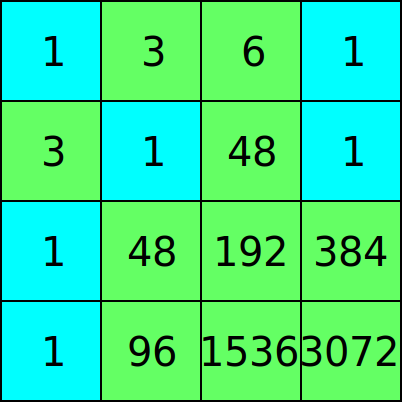
\includegraphics[width=0.35\textwidth]{figures/endboard.pdf}
	\caption{An example end-state board of \threes{}.}
\end{figure}

\threes{}\cite{threes} is a simple puzzle game involving a 4x4 grid, where the objective is to `slide' the tiles on the board such as to maximise the score according to a set of rules. This game was the basis of this project; to develop a program that could play a modified version of \threes{} at a rate of 5-10 moves per second.

While largely the same, rules concerning the placement of tiles and which tiles would be inserted after each slide were modified, making the game completely deterministic. In particular, the sequence of tiles which would be inserted after every move was known, and was always placed in the row with the lowest lexicographic score, or in the `most clockwise' row for the case of a tie.

\section{Prior work}\label{section:prior-work}
Being a relatively new game, the presence of pre-existing solvers was limited. Nonetheless, two works were considered --- one a solver for \threes{}\cite{tsolver}, and another a solver for a related game, \emph{2048}\cite{2048solver}. Both solutions used a minimax strategy with $\alpha$--$\beta$ pruning. As the modified version of \threes{} was deterministic, minimax was not an applicable solution. Still, it was found that of more importance was understanding \emph{how} these solvers distinguished good board states from bad ones.

\subsection{\threes{} solver} \label{threes-solver}
This solution uses a heuristic that considers the ``friction'' of a board, measuring how easy it is to combine adjacent tiles\cite{tsolver}. Boards which can freely combine adjacent tiles receive a lower ``friction'' compared to those where they are not combinable. The goal is therefore to prefer boards with a lower ``friction''.

Although this specific heuristic was not directly considered, it was found that in coming up with other heuristics, a similar train of thought was followed --- to maximise the number of combinable tiles on the board at any one time.

\subsection{2048-AI}\label{2048-solver}
While the game of \emph{2048} is not the same as \threes{}, its game mechanics share many similarities, which was why it was considered. Indeed, this similarity did lead to the discovery of some quite good heuristics that were also applicable to this game. Multiple heuristics were used, including:
\begin{enumerate}
	\singlespacing
	\item{The number of empty tiles present}
	\item{The ``smoothness'' of the board}
	\item{The ``monotonicity'' of the board}
	\item{The maximum value on the board}
	\onehalfspacing
\end{enumerate}

The author described in detail why such heuristics were used\cite{2048explanation}. Overall, it was found that the first two were particularly useful, while the latter two could not be successfully used. 

In experimentation, maximising the number of empty tiles was perhaps one of the most important characteristics of defining a ``good'' board. This was because having more free tiles allows for significantly greater freedom and flexibility when accommodating for new tiles. Implicitly, this heuristic has the effect of encouraging tiles to be combined where possible.

The second useful heuristic of ``smoothness'' was also important, but to a somewhat lesser extent. ``Smoothness'' is a measure of difference between adjacent tiles ---  boards are smoother where adjacent tiles have a similar value, compared to those where a large disparity exists. This has the effect of coalescing similar-valued tiles, making it easier to combine them when needed. It was interesting to note that the particular implementation of ``smoothness'' used in this project tended to gather high valued tiles in the corners; usually the lower right-hand corner.

``Monotonicity'' determines how well tiles increase in value monotonically along any row or column. This is to prevent a condition known as ``checkerboarding'', where high valued tiles alternate with low valued tiles. Checkerboarding is extremely undesirable, as it effectively prevents tiles from being combined, and can quite quickly lead to a premature end-state. Disappointingly, in testing it was found that a heuristic based on monotonicity did not have any significant effect. Instead, a different heuristic involving determining how many times a row or column changes from increasing to decreasing (and vice-versa) value was found to be more effective.

\subsection{Common player strategies}
In final consideration were the common strategies\cite{threes-strategies} players used to maximise their score. Apart from that already discussed, additional suggestions involved maximising the degrees of freedom (how many directions you can move in), and using the `corner' strategy of keeping large valued tiles in one corner. 

In general, it was found that the degrees of freedom at any board state did not change from four until you were about to approach a terminal state. This meant that the degrees of freedom was a good measure of when a board state was `bad', and should, if possible, be avoided. Although not intentional, the smoothness heuristic used also enforced the `corner strategy', as previously mentioned in Section~\ref{2048-solver}.

%-------------------------Candidate solutions----------------------

\section{Candidate methods to solving the modified version of \threes{}}
The fact that the modified game is deterministic heavily influenced the strategies considered for `solving' the game. As a result of the determinism, the game tree can theoretically be completely generated, using any common search strategy. This effectively brute-forces a solution by considering all possible board states. 

The only show-stopper to a brute-forced solution is that \threes{} has a branching factor of 4, since you can move in up to 4 directions (left, up, right, down). This makes a complete expansion of the game tree unfeasible, particularly for games with long tile sequences --- it is not uncommon to have a game that runs for in excess of 1000 moves. A complete search to that depth requires about 10\ts{602} nodes to be expanded; even at an expansion rate of 1ns/node, it would still take 10\ts{593} seconds, or about 10\ts{585} years.  

In reality, the maximum lookahead that can be reasonably achieved is to around a depth of 14, as required to achieve the solving speed of about 5--10 moves per second. It is possible that a greater lookahead could be achieved with the use of some form of pruning, hence preventing the expansion of nodes that are unlikely to lead to a good outcome.

Informed search strategies, such as A* were also considered to be possible, and would be desirable over uninformed search strategies, given that with the right heuristics, a good solution is likely to be found sooner. However, it is debatable whether or not an \emph{admissible} heuristic exists for this game. 

For both informed and uninformed search strategies, versions with more restricted memory usage (e.g. IDFS, SMA*, IDA*) could be used to overcome concerns over excessive memory usage.

\chapter{Implementation details}
The final solution implements two differing methods, with the first\footnote{This shall henceforth be referred to as `the first method' or `Method 1'} being a simple greedy algorithm that chooses the next best move according to some evaluation function, in combination with a fixed lookahead and some measure of backtracking. The second method\footnote{This shall henceforth be referred to as `the second method' or `Method 2'} can be described as an augmented version of the first implementation, and is closer in description to the A* algorithm. In particular, it maintains a \emph{fixed size} set of the most promising board states, where they are ordered by their $f$ value (in A* terminology), which is the sum of their heuristic evaluation and cost function (the number of moves made). As with the first method, this still expands the most promising node first, but the set of nodes that it maintains means that it can try alternate pathways much more flexibly when a dead-end occurs.

Both methods do not guarantee that \emph{the} optimal solution to be found, but it does usually find \emph{a} good solution. This is because both methods don't explore the full game tree, and depend quite heavily on the heuristic function to guide the algorithm in the correct direction. Further expanding on this, it can be seen why the second method is not an implementation of A* --- it only maintains a fixed size pool of unexplored nodes, and the heuristic used is not admissible.

\section{Determination of heuristics to be used}
Discerning which heuristics to use was difficult. As previously discussed in Section~\ref{section:prior-work}, prior work helped immensely to create useful heuristics. In any case, this process still required a fair amount of trial-and-error by simply observing what would happen if a particular heuristic was used. Over the course of this process, the following heuristics were considered:
\begin{enumerate}
	\singlespacing
	\item The current score of the board
	\item The average tile value of the board
	\item The median tile value of the board
	\item The number of tiles with value greater than three
	\item The number of tiles with value greater than the average
	\item The number of tiles with value greater than the median
	\item The number of tiles with value greater than the average
	\item The weighted sum of the number of combinable tiles
	\item Counting the number of time the sign changes along all rows/columns
	\item The degrees-of-freedom of the board
	\item The number of empty tiles on the board
	\item Counting the number of time the sign changes along all rows/columns and weighting it for larger differences
	\item The smoothness of the board
	\item The number of combinable tiles on the board
	\onehalfspacing
\end{enumerate}

In the end, only the last 5 heuristics (10-14) were used. Of special note is using the score of the board. While this is perhaps the most obvious heuristic, it was found to be problematic as it would often `drown out' the other heuristics, especially for long running boards with very high scores. Even when using the logarithm of the score, it did not often produce good results.

\section{Determination of heuristic weights}
The heuristics were combined using a linear weighting process. It was found that this step of determining what weights should be used was one of the most time consuming, because of the large range of possible weight combinations. While not being a particularly efficient method, the heuristic weights were found by simply enumerating all possible combinations and observing which ones produced the best results. This was then repeated on a number of boards to see which values worked best on most boards.

Part of the reason why this step took so long was that testing was based on the performance of the first method. This method was highly temperamental, and what weights worked well for one board, did not generally work as well on another. It was hypothesised that a dead-end could be typically resolved locally, and would only require to choose an alternate pathway from a few steps back to overcome the issue. Thus, limited backtracking was introduced to help overcome this problem, where the agent could move back a fixed number of steps and re-evaluate the nodes using a different set of heuristic weights. While this did help quite substantially, performance was still found to vary quite markedly from board to board.

Dissatisfaction in the variability of performance was why the second method was authored, and in doing so, it was found that the sensitivity to what heuristic weights were used was greatly reduced.

\section{Performance analysis}
The first method has no feedback, so the run-time of this method will vary from board to board, and can vary significantly from computer to computer. The worst-case running time for this algorithm is proportional to $O(k(b^n))$ where $b$ is the branching factor (4), $n$ is the lookahead depth limit (8) and $k$ is the number of tiles in the sequence. This corresponds to where a complete depth-first search to a depth 8 is required for each move of 8 steps.

The second method does incorporate a feedback mechanism, so it will usually have a worst-case runtime of 5 moves/second, which is practically guaranteed when run on any modern computer. On computers which are not modern (i.e. Pentium 4 or lower; the computer that this was developed on), performance can fall below 5 moves/second.

Multi-threading was also introduced fairly late, but it did help to significantly increase the solving speed --- often by a factor of two, where the resources are available. This was achieved by splitting the game tree into 4 subtrees (by moving in the 4 directions) and searching each of the 4 subtrees in parallel. However, this design means that it will use at most 4 (logical) cores, and will often slightly under-utilise them, given that the game tree is not balanced.

Memory usage is not a concern for either method, as they both use a depth first search which has a space complexity of $O(bn)$. Additionally, the second method does not suffer from the memory issues of A* as its node pool is fixed in size. Typically, the solver will use no more than 400MB of RAM.

\section{Experimental results}
Experimentation was conducted on the Undergraduate CSSE SSH server (GP05), which has an Intel Xeon E5-2640 (2.50GHz) and 2GB of usable RAM. As enforced by the server, CPU utilisation was restricted to two cores.

For both methods, it is typical to expect it to solve to at least 1000 moves, but this is notwithstanding boards where it is particularly difficult to select good moves. In cases where the tile sequence is unfavourable, it may be found that it will solve no more than 200 moves. Such boards are ones where there is a very high proportion of low valued (1 or 2) tiles, and where such tiles occur in long sequences that makes them uncombinable. The presence of such uncombinable tiles severely limits the performance of the solver, as they quickly fill the board and do not significantly contribute to its score.

However, on boards where the tile sequence is favourable (easily combinable), it has been shown that this solver can continue for many thousands of moves quite easily. The second method in particular will usually run sequences to completion or near completion when possible. It should be noted that any agent will not perform well if a long sequence of uncombinable tiles occurs. 

Irregardless, the second method is used by default, with the first usable only by explicit command. The first method was retained simply because a lot of time was spent on this option, and the second method was only added quite late into the project.

\subsection{Test boards}
\begin{table}[H]
  \centering
  \caption{The test boards used}
    \begin{tabular}{|l|c|ccc|cccccc|}
    \hline
          &       & \multicolumn{3}{c|}{Maximum continuity}  & \multicolumn{6}{c|}{Tile proportion (\%)} \\
    Board name & Tile count & Tile value & Length & Position & 1     & 2     & 3     & 6     & 12    & 24 \\
    \hline
    \texttt{exampleinput.txt} & 32    & 3     & 2     & 3     & 25.0  & 28.1  & 34.4  & 6.2   & 6.2   &  -- \\
    \texttt{B1.txt} & 74    & 2     & 3     & 44    & 44.6  & 37.8  & 16.2  & -- & 1.4   & --  \\
    \texttt{short-range.txt} & 500   & 1     & 10    & 116   & 43.0  & 41.6  & 7.8   & 4.8   & 2.8   & -- \\
    \texttt{medium-range.txt} & 1000  & 1     & 7     & 340   & 46.2  & 45.7  & 3.9   & 4.7   &  --     & -- \\
    \texttt{long-range.txt} & 2000  & 1     & 8     & 1947  & 40.4  & 40.7  & 7.5   & 4.2   & 3.6   & 3.5 \\
    \texttt{longboard-1.txt}\tablefootnote{Also known as \texttt{evan.in} \cite{help3001-boards}} & 20000 & 1     & 9     & 3727  & 40.1  & 40.1  & 9.8   & 3.2   & 3.3   & 3.4 \\
    \texttt{longboard-2.txt}\tablefootnote{Also known as \texttt{ridge.in} \cite{help3001-boards}} & 4000  & 2     & 6     & 3109  & 33.4  & 33.3  & 33.3  &  --     &  --     & -- \\
    \texttt{longboard-3.txt}\tablefootnote{Also known as \texttt{eliot.in} \cite{help3001-boards}} & 20000 & 4     & 2     & 82    & 40.0  & 40.0  & 9.9   & 3.4   & 3.4   & 3.3 \\
    \hline
    \end{tabular}%
  \label{tab:test-boards}%
\end{table}%

With these boards, three primary tests were conducted --- one using method 1, one using method 2 with default settings, and one using method 2 with faster settings. Method 2 is highly user configurable (see Appendix~\ref{appendix-manual}), with options affecting the final result achieved and the speed at which a result is produced.

\begin{table}[H]
  \centering
  \caption{Test results using method 1}
    \begin{tabular}{lrrr}
    \hline
    Board name & Final score & Tile utilisation & Speed (moves/second) \\
    \hline
    \texttt{exampleinput.txt} & 773   & 32/32 & 34.08 \\
    \texttt{B1.txt} & 1012  & 74/74 & 40.42 \\
    \texttt{short-range.txt} & 22180 & 488/500 & 58.83 \\
    \texttt{medium-range.txt} & 7724  & 336/1000 & 31.91 \\
    \texttt{long-range.txt} & 27072 & 440/2000 & 55.98 \\
    \texttt{longboard-1.txt} & 259164 & 2100/20000 & 72.53 \\
    \texttt{longboard-2.txt} & 593530 & 4000/4000 & 39.97 \\
    \texttt{longboard-3.txt} & 6635430 & 14784/20000 & 40.87 \\
    \hline
    \end{tabular}%
  \label{tab:results-method1}%
\end{table}%

\begin{table}[H]
  \centering
  \caption{Test results using method 2 with default settings}
    \begin{tabular}{lrrr}
    \hline
    Board name & Final score & Tile utilisation & Speed (moves/second) \\
    \hline
    \texttt{exampleinput.txt} & 773   & 32/32 & 5.25 \\
    \texttt{B1.txt} & 1012  & 74/74 & 5.20 \\
    \texttt{short-range.txt} & 22257 & 500/500 & 39.82 \\
    \texttt{medium-range.txt} & 61274 & 1000/1000 & 21.99 \\
    \texttt{long-range.txt} & 29530 & 530/2000 & 4.52 \\
    \texttt{longboard-1.txt} & 259164 & 2100/20000 & 11.35 \\
    \texttt{longboard-2.txt} & 593530 & 4000/4000 & 27.29 \\
    \texttt{longboard-3.txt} & 14968605 & 20000/20000 & 34.80 \\
    \hline
    \end{tabular}%
  \label{tab:results-method2-default}%
\end{table}%

\begin{table}[H]
  \centering
  \caption{Test results using method 2 with \texttt{-a 4 -u 300 -q 20000}}
    \begin{tabular}{lrrr}
    \hline
    Board name & Final score & Tile utilisation & Speed (moves/second) \\
    \hline
    \texttt{exampleinput.txt} &   773    &   32/32    & 18.53  \\
    \texttt{B1.txt} &   1012    &  74/74     &  61.63 \\
    \texttt{short-range.txt} & 22284 & 500/500 & 303.43 \\
    \texttt{medium-range.txt} & 61274 & 1000/1000 & 164.70 \\
    \texttt{long-range.txt} & 29530 & 530/2000 & 31.60 \\
    \texttt{longboard-1.txt} & 259164 & 2100/20000 & 117.91 \\
    \texttt{longboard-2.txt} & 593529 & 4000/4000 & 1127.62 \\
    \texttt{longboard-3.txt} & 642924 & 14952/20000 & 362.51 \\
    \hline
    \end{tabular}%
  \label{tab:results-method2-modded}%
\end{table}%

It should be quite clear that while method 1 has a fairly consistent speed, it fails to perform well in all situations. The second method produces much better results in that it is consistently able to use more tiles and continue further than method 1. Method 2 does tend to run slower on boards with low tile counts (e.g. \texttt{exampleinput.txt}), or boards where it gets stuck (e.g. \texttt{long-range.txt}), but the effect of the feedback system is shown, where the minimal speed is around 5 moves/second.

Quite surprisingly, method 2 performs unexpectedly well even with a low lookahead, as seen in Table~\ref{tab:results-method2-modded}. In fact, using these settings, it is on average 12 times faster than with default settings, and produces exactly the same results, except for two cases --- \texttt{longboard-2.txt} and \texttt{longboard-3.txt}. For \texttt{longboard-2.txt}, it still uses 4000/4000 tiles, but scores one point less, which is a practically negligible difference. For \texttt{longboard-3.txt}, the difference in score is more apparent, but it still manages to outperform method 1 at almost 10 times the speed.

\begin{figure}[H]
	\centering
	\resizebox{0.8\textwidth}{!}{\import{figures/}{figure_1.pgf}}
	\caption{A plot comparing the running speed to the lookahead depth (method 2).}
	\label{fig:lookahead_speed}
\end{figure}

\begin{figure}[H]
	\centering
	\resizebox{0.8\textwidth}{!}{\import{figures/}{figure_2.pgf}}
	\caption{A plot comparing the tile usage to the lookahead depth for boards where it varied.}
	\label{fig:lookahead_tileusage}
\end{figure}

\begin{figure}[H]
	\centering
	\resizebox{\textwidth}{!}{\import{figures/}{figure_3.pgf}}
	\caption{A plot comparing the score to the lookahead depth.}
	\label{fig:lookahead_score}
\end{figure}

For these graphs, the solver was run with the following settings:
\begin{itemize}
	\singlespacing
	\item For lookahead \texttt{x} in range 1-5: \texttt{-a x -u 220 -q 30000}
	\item For lookahead \texttt{x} in range 6-7: \texttt{-a x -u 220 -q 20000}
	\item For lookahead of 8 (default): No options
	\onehalfspacing
\end{itemize}

What is quite apparent is that the lookahead has a minimal effect on the end result, except for those with very long tile sequences (i.e. in excess of 10,000 pieces). As seen in Figure~\ref{fig:lookahead_speed}, the solving speed decreases by orders of magnitude as the lookahead is increased (the y-axis is logarithmic). This suggests that it is better to use a lower lookahead to quickly gauge how many moves a board can be solved for, before using a higher lookahead to get the best results. 

In conclusion, method 2 should always be used over method 1, and the lookahead depth used by method 2 can be safely dropped to increase speed, with minimal effect on the final result. 

\chapter{Potential areas for improvement}
Over the course of development there were several key areas that could have been further refined to get better results.

\begin{itemize}
	\item Both methods do not make use of caching, and must generate the game tree again if it needs to re-search part of it (backtracking)
	\item Visited nodes are not kept track of, which leads to re-evaluation of nodes when the solver is stalled (method 2)
	\item When method 2 gets stalled, it tends to explore all nodes close to the stall point first, instead of backtracking further to a point where it is more likely to get out of the stall. As the queue size is restricted, this behaviour can tend to `flood-out' the queue with nodes too close to the stall, making it impossible to get past it. 
	
	At present, this is partially limited by the behaviour of simply dropping the top half of the queue of nodes to explore, if it is detected that the solver is stalled. However, this is a `dumb' method, as it doesn't explicitly consider which node would be best to backtrack to.
	\item The depth limited search used for lookahead has a fixed cutoff based on the depth of exploration only. A better implementation would also consider the board state to determine if more or less searching is required (variable cutoff).
	\item The heuristics used and their weights may need tweaking to get better results. One way this could be achieved is to consider the determination of heuristic weights as a mathematical optimisation problem, with the goal being to maximise the final score. Multiple optimisation algorithms exist to solve such a problem\cite{scipy-optimisation}.
	\item The backing data structure of the size-limited priority queues is a balanced binary tree (TreeSet), which allows for the ordering of elements and $O(log(n))$ performance to add and remove any of its elements. This means that least-valued nodes can be easily pruned (i.e. the tail-end of the queue) to maintain a fixed size. However, elements in the middle cannot be easily accessed without knowing in advance what is currently there. This prevents efficient backtracking to elements further down the queue if a stall occurs.
	\item Profiling\footnote{See Appendix~\ref{appendix-profiling}} the solver seems to suggest that most of the memory usage is from copying the string of moves made with each new board. If memory usage was a concern, a smarter method of keeping track of the moves made may be of use.
	\item Additional profiling suggests that most of the calculation time is spent in either copying the boards (initialisation of the moves string) or updating of the priority queue (TreeSet). Targeting these areas, alternative data structures and/or alternative methods may help to increase performance.
\end{itemize}


%Appendix
%---------------------------------------------------------
\begin{appendices}
%Override issues with using appendix with titlesec
\renewcommand{\chaptername}{Appendix}
\renewcommand{\chaptermark}[1]{\markboth{\chaptername~\thechapter~~#1}{}}
\titleformat{\chapter}
	{\normalfont\LARGE\bfseries}{\chaptername~\thechapter.}{0.8em}{}
%---------------------------------------------------------

\chapter{Solver documentation}\label{appendix-manual}
The solver is written in Java, and requires the Java runtime version 7 or later to function. On most platforms, the usual way to call the program is with:
\begin{lstlisting}
        java -jar threes.jar [options] input_file.txt
\end{lstlisting}

On Windows, a convenience launcher exists, such that it can be called by:
\begin{lstlisting}
        Threes.exe [options] input_file.txt
\end{lstlisting}

The output moves file is always written to \texttt{stdout}. All other messages should be written to \texttt{stderr}.

\begin{table}[H]
  \centering
  \caption{A list of user-configurable options}
    \begin{tabularx}{\textwidth}{lX}
    \hline
    Command & Description \\
    \hline
    \texttt{-v} & Enables verbose output to \texttt{stderr}. Highly recommended, as it shows the progress and state of the solver at any one time. \\
    \texttt{-s} & Switches to single-threaded mode. May be useful if multi-threading causes issues (it shouldn't). \\
    \texttt{-d} & Switches to using method 1 as the solving algorithm. \\
    \texttt{-n} & Disables backtracking in method 1. \\
    \texttt{-l <i,j,k,l>} & Enables `learning' mode, which uses method 1 as the solver for the input board. It iterates over all possible heuristic weights and repeatedly solves the board. Results are displayed so that the user can see what weights work well. The four comma separated integer values, \texttt{i,j,k,l} indicate the starting weights. \\
    \texttt{-a <n>} & Controls the lookahead depth. The default value is 8, which produces the best results overall in a reasonable time. Lesser depths (e.g. n=4) increases the speed by an order magnitude and the results generally remain good too.  \\
    \texttt{-u <n>} & Controls the main priority queue size. The default is 200, and should be increased (to about 300) for depths less than 8. Increasing this too much may cause it to get stuck examining lower valued boards instead of continuing. \\
    \texttt{-i <n>} & Controls the nominal size of individual priority queues. In essence, it controls how many nodes are added to the main queue after each iteration of lookahead/evaluation. The default value is 2, and in general does not need to be changed. This value is nominal, as when the main queue is nearly empty, the size is automatically increased to populate the main queue quickly. \\
    \texttt{-q <n>} & Controls the `quiescence' limit. This number represents how many iterations the best result has remained the same for (i.e. are we stalled?). The default value is 5000. For depths less than 8, it is recommended to increase this to about 20,000 or more. Increasing this value too much will cause it to run slower as it tries more possibilities when stalled, but the speed should not fall below 5 moves/second. Too low however, and the agent may prematurely end without considering a path to get past the stall.\\
    \texttt{-o <output\_file>} & In addition to writing the output to \texttt{stdout}, the output will also be written to the specified output file. \\
    \texttt{-m <moves\_file>} & Reads in the moves file and plays that board repeatedly. For benchmarking purposes only. \\
    \hline
    \end{tabularx}%
  \label{tab:method2-parameters}%
\end{table}%

\section{An explanation of the verbose output}
When run in verbose mode, the output will typically look something like this:
\begin{lstlisting}
PQ Size: 199 (0)
88635 (1032)
 12   0   1   2
  6  12  24  48
  6  12 192 768
  1  96 384 1536
\end{lstlisting}

\begin{itemize}
\item At line 1: \texttt{199} indicates that the main priority queue currently holds 199 candidate boards. The bracketed number, \texttt{(0)}, indicates the number of times that the current best solution has not changed from. If this number increases from 0, it usually indicates that the solver `stalled' and had to backtrack to try an alternate pathway. If this number reaches the quiescence limit, then solving will halt and the current best solution is returned.
\item At line 2: The first number, \texttt{88635}, indicates the board score of the board currently being explored. The bracketed number, \texttt{(1032)} indicates the number of moves that has been made so far for the current board. 
\item Lines 3-6: The current board state.
\end{itemize}

\chapter{Profiling the application in NetBeans}\label{appendix-profiling}
This profiling was conducted using NetBeans 7.4 with JRE version 1.7 on the lab computers in CSSE 2.03.

\begin{figure}[H]
	\centering
	\includegraphics[width=0.85\textwidth]{figures/Speed-profiling.png}
	\caption{Speed profiling reveals the breakdown of CPU time spent in each method.}
	\label{fig:speed-profiling}
\end{figure}

\begin{figure}[H]
	\centering
	\includegraphics[width=0.85\textwidth]{figures/Memory-profiling.png}
	\caption{Memory profiling reveals the breakdown of memory allocation.}
	\label{fig:memory-profiling}
\end{figure}

\end{appendices}

%---------------------------------------------------------
%Referencing
%---------------------------------------------------------
\renewcommand{\bibname}{References}
\bibliography{references/refs}
\bibliographystyle{ieeetr}  
\addcontentsline{toc}{part}{References}
%---------------------------------------------------------

\end{document}